\documentclass[tikz,border=6pt]{standalone}
\usepackage{pgfplots}
\pgfplotsset{compat=1.18}
\definecolor{demand}{HTML}{1F4E79}
\definecolor{mr}{HTML}{7EA6C8}
\definecolor{mc}{HTML}{B23A32}
\definecolor{point}{HTML}{C5161D}
\definecolor{profit}{HTML}{7BC99A}
\begin{document}
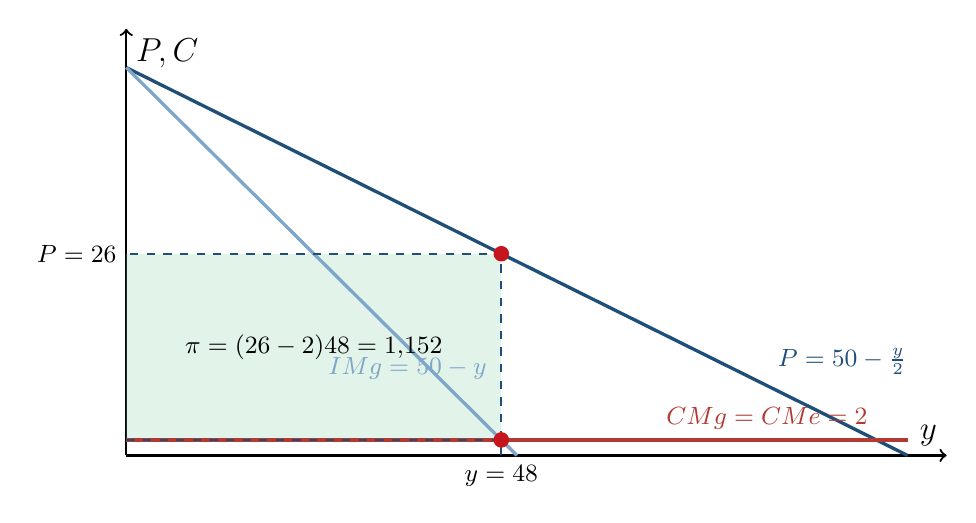
\begin{tikzpicture}
\begin{axis}[width=12cm,height=7cm,axis lines=middle,xmin=0,xmax=105,ymin=0,ymax=55,xtick=\empty,ytick=\empty,xlabel={$y$},ylabel={$P,C$},axis line style={->,thick},label style={font=\large},tick style={draw=none},clip=false]
\path[fill=profit,opacity=.22] (axis cs:0,2) rectangle (axis cs:48,26);
\addplot[domain=0:100,samples=2,very thick,demand] {50-.5*x} node[pos=.82,above right,font=\small] {$P=50-\frac{y}{2}$};
\addplot[domain=0:50,samples=2,very thick,mr] {50-x} node[pos=.72,below,font=\small] {$IMg=50-y$};
\addplot[domain=0:100,samples=2,very thick,mc] {2} node[pos=.82,above,font=\small] {$CMg=CMe=2$};
\addplot[dashed,thick,demand] coordinates {(48,0) (48,26) (0,26)};
\addplot[dashed,thick,demand] coordinates {(0,2) (48,2)};
\addplot[only marks,mark=*,mark size=2.6pt,point] coordinates {(48,26) (48,2)};
\node[left,font=\small] at (axis cs:0,26) {$P=26$};
\node[below,font=\small] at (axis cs:48,0) {$y=48$};
\node[font=\small] at (axis cs:24,14) {$\pi=(26-2)48=1{,}152$};
\end{axis}
\end{tikzpicture}
\end{document}
